\documentclass[11pt]{article}
\usepackage[margin=1in]{geometry}
\usepackage{amsmath,amssymb,bm}
\usepackage[T1]{fontenc}
\usepackage[utf8]{inputenc}
\usepackage{lmodern}
\usepackage{booktabs}
\usepackage{longtable}
\usepackage{array}
\usepackage{enumitem}
\usepackage{hyperref}
\usepackage{tikz}
\usetikzlibrary{arrows.meta,positioning,calc,shapes.geometric}

\title{Road Event Detector Formulations}
\author{road\_events documentation}
\date{\today}

\newcommand{\dt}{\Delta t}
\newcommand{\abs}[1]{\left|#1\right|}
\newcommand{\sgn}{\operatorname{sgn}}

\begin{document}
\maketitle
\tableofcontents
\newpage

\section{Scope}

This document records the math and streaming algorithms implemented by the
\path{road_events} crate. The crate detects road events from vehicle-frame
motion signals produced by the simulation and visualization pipeline. The
detectors are intentionally small-state and embedded-friendly: they process one
sample at a time, use bounded memory, and avoid FFTs, dynamic allocation, and
offline window buffering.

The detectors are not part of the EKF state estimator. They consume already
estimated or referenced motion channels such as vehicle speed, vehicle pitch,
gravity-compensated vertical acceleration, and vehicle-frame lateral specific
force. The current event set is:
\begin{itemize}[nosep]
  \item speed bumps,
  \item sustained uphill and downhill intervals,
  \item reverse-driving intervals,
  \item harsh acceleration,
  \item harsh braking,
  \item harsh cornering,
  \item road-surface roughness and rough-road intervals,
  \item short vertical road shocks,
  \item streaming trip statistics such as distance, duration, speed extrema,
    elevation gain/loss, and event rates.
\end{itemize}

\section{Signals and Units}

\begin{longtable}{>{\raggedright\arraybackslash}p{0.22\linewidth} >{\raggedright\arraybackslash}p{0.20\linewidth} >{\raggedright\arraybackslash}p{0.48\linewidth}}
\toprule
\textbf{Symbol} & \textbf{Unit} & \textbf{Meaning} \\
\midrule
\(t_k\) & s & Sample timestamp. \\
\(v_x\) & m/s & Vehicle-frame forward velocity. Positive is forward; negative is reverse. \\
\(s=\abs{v_x}\) & m/s & Speed magnitude used by threshold logic. \\
\(\theta\) & deg & Vehicle pitch angle. Positive pitch is uphill in the current detector convention. \\
\(a_z\) & m/s\(^2\) & Gravity-compensated vehicle-frame vertical acceleration. \\
\(a_{z,\mathrm{bp}}\) & m/s\(^2\) & Band-passed vertical acceleration used for road roughness. \\
\(a_y\) & m/s\(^2\) & Vehicle-frame lateral specific force. Positive is to vehicle right. \\
\bottomrule
\end{longtable}

The speed-bump detector uses pitch and vertical acceleration. Road roughness
uses gravity-compensated vertical acceleration and speed. Hill detection uses
pitch and speed. Reverse and harsh longitudinal detection use forward velocity.
Harsh cornering uses speed and vehicle-frame lateral specific force. Trip
statistics consume the same vehicle-motion stream and update running totals
without storing history.

\begin{figure}[h]
\centering
\vspace{0.4cm}
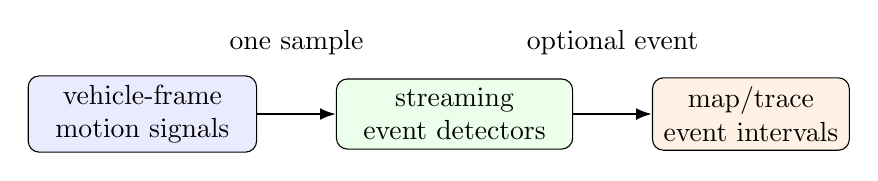
\begin{tikzpicture}[
  node distance=0.85cm and 1.0cm,
  src/.style={draw,rounded corners,fill=blue!8,align=center,minimum width=2.9cm,minimum height=0.75cm},
  det/.style={draw,rounded corners,fill=green!8,align=center,minimum width=3.0cm,minimum height=0.75cm},
  eventnode/.style={draw,rounded corners,fill=orange!10,align=center,minimum width=2.5cm,minimum height=0.75cm},
  arr/.style={-{Latex[length=2mm]},thick}
]
  \node[src] (motion) {vehicle-frame\\motion signals};
  \node[det,right=of motion] (detectors) {streaming\\event detectors};
  \node[eventnode,right=of detectors] (events) {map/trace\\event intervals};
  \draw[arr] (motion) -- node[above=7mm,fill=white,inner sep=1pt]{one sample} (detectors);
  \draw[arr] (detectors) -- node[above=7mm,fill=white,inner sep=1pt]{optional event} (events);
\end{tikzpicture}
\caption{All event detectors run as streaming post-processors over vehicle
motion signals.}
\end{figure}

\section{Shared Streaming Primitives}

\subsection{Timestamp Handling}

The implementation clamps per-sample time deltas to keep bad or repeated
timestamps from creating unbounded filter updates:
\begin{equation}
  \dt_k = \operatorname{clamp}(t_k-t_{k-1}, 0, 0.2).
\end{equation}
For high-pass and derivative paths that require a strictly positive time step,
the lower bound is \(10^{-3}\) or \(10^{-4}\) seconds depending on the path.

\subsection{First-Order High-Pass Filter}

The speed-bump detector removes road grade and slow body motion with the
standard discrete first-order high-pass filter:
\begin{align}
  \tau &= \frac{1}{2\pi f_c},\\
  \alpha_k &= \frac{\tau}{\tau+\dt_k},\\
  y_k &= \alpha_k(y_{k-1}+u_k-u_{k-1}).
\end{align}
This is applied independently to vehicle pitch and gravity-compensated vertical
acceleration.

\subsection{Exponential Moving Average}

The crate uses an exponential moving average (EMA) for adaptive noise floors
and smoothed velocity derivatives:
\begin{align}
  \alpha_k &= \frac{\dt_k}{\max(\tau,\dt_k)+\dt_k},\\
  \bar{x}_k &= (1-\alpha_k)\bar{x}_{k-1}+\alpha_k x_k .
\end{align}
For noise floors, the input is the absolute high-pass value:
\begin{equation}
  \sigma_k = \operatorname{EMA}(\sigma_{k-1}, \abs{y_k}, \tau, \dt_k).
\end{equation}
The EMA is a low-memory substitute for a sliding RMS window. It provides slow
adaptation to background vibration without storing historical samples.

\subsection{Distance-Domain EMA}

Road roughness should compare road surface quality over distance rather than
over wall-clock time. For a distance increment
\begin{equation}
  \Delta s_k = s_k\Delta t_k,
\end{equation}
the crate uses a first-order distance-domain EMA:
\begin{equation}
  \alpha_k = \frac{\Delta s_k}{L+\Delta s_k},
  \qquad
  E_k = (1-\alpha_k)E_{k-1}+\alpha_k e_k .
\end{equation}
This is the same small-state first-order update as the time-domain EMA, but the
independent variable is traveled distance. \(L\) is the effective road interval
length. The default \(L=10~\mathrm{m}\) makes the estimate close to continuous:
roughness rises over locally rough pavement and dissipates quickly after the
vehicle returns to clean road, without requiring a rolling buffer.

\subsection{Interval Accumulation}

Most detectors convert an instantaneous metric \(m_k\) into an event interval
using enter and exit thresholds:
\begin{align}
  \text{enter if}\quad &m_k \ge m_{\mathrm{enter}},\\
  \text{stay active while}\quad &m_k \ge m_{\mathrm{exit}},
  \qquad m_{\mathrm{exit}} < m_{\mathrm{enter}}.
\end{align}
During an active interval the detector accumulates:
\begin{align}
  T &= \sum_k \dt_k,\\
  \bar{m} &= \frac{1}{T}\sum_k m_k\dt_k,\\
  m_{\max} &= \max_k m_k,\\
  \bar{s} &= \frac{1}{T}\sum_k s_k\dt_k.
\end{align}
The interval is emitted only if \(T\ge T_{\min}\). A refractory time suppresses
duplicate events immediately after a valid event.

\section{Road Roughness Analyzer}

\subsection{Metric}

\path{RoadRoughnessAnalyzer} estimates continuous road-surface roughness and
also emits two event types from the same vertical-motion stream:
\begin{itemize}[nosep]
  \item rough-road intervals for sustained increases in ambient road texture,
  \item road-shock intervals for short isolated vertical impacts such as sharp
    joints, potholes, or large bump impulses.
\end{itemize}

The input is vehicle-frame, gravity-compensated vertical acceleration. The
implementation first rejects grade, body attitude drift, and high-frequency
sensor/structure noise:
\begin{align}
  a_{z,\mathrm{hp},k} &=
    \operatorname{HPF}(a_{z,k}; f_c=0.7~\mathrm{Hz}),\\
  a_{z,\mathrm{bp},k} &=
    \operatorname{LPF}(a_{z,\mathrm{hp},k}; f_c=10~\mathrm{Hz}).
\end{align}
Before the first ambient baseline is available, the limiter uses a conservative
minimum cap. Afterwards, large isolated defects are hard-limited before they
enter the roughness energy:
\begin{equation}
  C_k = \min\left(1.5,\max(0.6,3B_{k-1})\right),
  \qquad
  \tilde{a}_{z,k}
  = \operatorname{clamp}(a_{z,\mathrm{bp},k}, -C_k, C_k).
\end{equation}
The analyzer then tracks a local ambient vibration baseline from the robust
band-passed magnitude:
\begin{equation}
  B_k = \operatorname{EMA}_{d}(B_{k-1}, \abs{\tilde{a}_{z,k}}, L_B),
  \qquad L_B=20~\mathrm{m}.
\end{equation}
The roughness energy sample is
\begin{equation}
  e_k = \tilde{a}_{z,k}^2 .
\end{equation}
When \(s_k\ge2.0~\mathrm{m/s}\), the analyzer updates the distance-domain
energy estimate with \(L=10~\mathrm{m}\):
\begin{equation}
  E_k = (1-\alpha_k)E_{k-1}+\alpha_k e_k,
  \qquad
  \alpha_k=\frac{s_k\Delta t_k}{10+s_k\Delta t_k}.
\end{equation}
When speed is below the gate, filter state is kept current but roughness energy
and valid roughness distance are held. This prevents stationary vibration and
parking-lot maneuvering from being interpreted as road texture.

The reported roughness is
\begin{equation}
  R_k = \sqrt{E_k}.
\end{equation}
Initial qualitative bands are:
\begin{center}
\begin{tabular}{lll}
\toprule
Class & Condition & Interpretation \\
\midrule
Very smooth & \(R<0.15~\mathrm{m/s^2}\) & Minimal vertical vibration. \\
Smooth & \(0.15\le R<0.25~\mathrm{m/s^2}\) & Low vertical vibration. \\
Light texture & \(0.25\le R<0.40~\mathrm{m/s^2}\) & Mild road texture. \\
Moderate & \(0.40\le R<0.60~\mathrm{m/s^2}\) & Noticeable sustained texture. \\
Rough & \(0.60\le R<0.90~\mathrm{m/s^2}\) & Sustained rough pavement. \\
Very rough & \(0.90\le R<1.20~\mathrm{m/s^2}\) & Strong sustained vibration. \\
Severe & \(R\ge1.20~\mathrm{m/s^2}\) & Extreme sustained vibration. \\
\bottomrule
\end{tabular}
\end{center}

\subsection{Why Not Peak Acceleration}

Peak vertical acceleration is already used by speed-bump detection. Roughness is
intended to describe a road interval, so a single bump or pothole should not
dominate the estimate. The band-pass, adaptive hard limiter, speed gate, and
10 m distance-domain EMA make the metric local and streaming while keeping
memory use constant.

\subsection{Rough-Road Events}

The continuous roughness estimate is also converted into a sparse event when
there is a sustained local uptick:
\begin{align}
  \text{enter if}\quad &R_k \ge 0.60~\mathrm{m/s^2},\\
  \text{remain active while}\quad &R_k \ge 0.42~\mathrm{m/s^2}.
\end{align}
The streaming analyzer distinguishes live notification from completed interval
reporting. A live notification is emitted as soon as the active interval reaches
one second, so embedded or UI consumers can react promptly. The completed
rough-road interval is emitted when \(R_k\) falls below the exit threshold or
when the stream is explicitly flushed. The completed interval is the one used
for offline map and trace analysis because its end time, duration, mean
roughness, peak roughness, mean speed, and distance are known. An eight-second
refractory period prevents repeated live notifications while the same rough
patch remains active.

\subsection{Road-Shock Events}

Road shocks use the raw band-passed magnitude before robust limiting, so
isolated high-energy impacts can be reported without contaminating the ambient
roughness estimate. The enter threshold is the larger of a fixed physical floor
and the local baseline-scaled threshold:
\begin{equation}
  A_{\mathrm{shock},k}
  = \max\left(2.5~\mathrm{m/s^2},\,6B_k\right).
\end{equation}
A shock candidate starts when
\(\abs{a_{z,\mathrm{bp},k}}\ge A_{\mathrm{shock},k}\) and remains active until
the magnitude falls below \(0.45A_{\mathrm{shock},k}\). It is emitted only if
its duration is between \(0.02\) and \(0.65~\mathrm{s}\). This separates sharp
impacts from sustained rough pavement. A \(0.5~\mathrm{s}\) refractory period
suppresses duplicate shock events from the same impulse sequence.

\section{Speed-Bump Detector}

\subsection{Physical Signature}

A road speed bump creates a short vertical impulse sequence as the front axle
and rear axle traverse the bump. In gravity-compensated vehicle-frame vertical
acceleration, the idealized pattern is an alternating sequence of three extrema:
\begin{equation}
  a_{z,\mathrm{hp}}(t_1),\quad a_{z,\mathrm{hp}}(t_2),\quad a_{z,\mathrm{hp}}(t_3),
  \qquad
  \sgn(a_1)=\sgn(a_3)\ne\sgn(a_2).
\end{equation}
Pitch motion is used as corroboration rather than as the primary trigger,
because pitch angle alone can also respond to braking, turning on uneven roads,
or grade changes.

\subsection{Filtered Signals}

The detector computes:
\begin{align}
  \theta_{\mathrm{hp},k} &= \operatorname{HPF}(\theta_k; f_c=0.45~\mathrm{Hz}),\\
  a_{\mathrm{hp},k} &= \operatorname{HPF}(a_{z,k}; f_c=0.70~\mathrm{Hz}).
\end{align}
Adaptive noise floors are:
\begin{align}
  \sigma_{\theta,k} &= \operatorname{EMA}(\abs{\theta_{\mathrm{hp},k}};\tau=6~\mathrm{s}),\\
  \sigma_{a,k} &= \operatorname{EMA}(\abs{a_{\mathrm{hp},k}};\tau=6~\mathrm{s}).
\end{align}
The peak thresholds are:
\begin{align}
  A_{\mathrm{thr}} &= \max(3.5\,\sigma_a,\;1.5~\mathrm{m/s^2}),\\
  \Theta_{\mathrm{thr}} &= \max(3.0\,\sigma_\theta,\;0.25^\circ).
\end{align}

\subsection{Extremum Extraction}

The vertical acceleration slope is
\begin{equation}
  \dot{a}_{\mathrm{hp},k}
  = \frac{a_{\mathrm{hp},k}-a_{\mathrm{hp},k-1}}{\dt_k}.
\end{equation}
A local maximum is detected when \(\dot{a}_{k-1}>0\) and \(\dot{a}_{k}\le 0\);
a local minimum is detected when \(\dot{a}_{k-1}<0\) and \(\dot{a}_{k}\ge 0\).
An extremum is kept only when its absolute vertical acceleration exceeds the
physical floor \(1.5~\mathrm{m/s^2}\). The detector stores only the latest four
extrema, so memory use remains constant.

For each extremum interval, the detector also stores the maximum pitch
high-pass magnitude since the previous extremum:
\begin{equation}
  \Theta_i = \max_{t\in(t_{i-1},t_i]}\abs{\theta_{\mathrm{hp}}(t)}.
\end{equation}

\subsection{Candidate Timing}

Each latest-three-extrema group is scored only if the polarities alternate. Let
\begin{equation}
  D = t_3-t_1,\qquad
  \bar{s}=\frac{s_1+s_2+s_3}{3}.
\end{equation}
The candidate must pass both absolute and speed-adaptive duration bounds:
\begin{align}
  D_{\min} &=
  \max\left(0.18,\;0.35\frac{L_{\min}}{\bar{s}}\right),\\
  D_{\max} &=
  \min\left(1.8,\;2.5\frac{L_{\max}}{\bar{s}}\right),
\end{align}
where \(L_{\min}=1.8~\mathrm{m}\) and \(L_{\max}=3.6~\mathrm{m}\) are plausible
front/rear axle spacing bounds. The speed must also satisfy
\(\bar{s}\ge1.5~\mathrm{m/s}\).

The detector tracks the total time within the pattern for which
\(\abs{a_{\mathrm{hp}}}\ge1.5~\mathrm{m/s^2}\). It requires:
\begin{align}
  T_{\mathrm{active}} &\ge 0.25~\mathrm{s},\\
  \frac{T_{\mathrm{active}}}{D} &\ge 0.25.
\end{align}

\subsection{Score and Confidence}

For extrema magnitudes \(A_i=\abs{a_i}\), pitch peaks \(\Theta_i\), and
candidate duration \(D\), the component scores are:
\begin{align}
  A_{\max} &= \max_i A_i,\\
  \Theta_{\max} &= \max_i \Theta_i,\\
  S_a &= \operatorname{clamp}\left(\frac{A_{\max}}{A_{\mathrm{thr}}}-1,\;0,\;1\right),\\
  S_\theta &= \operatorname{clamp}\left(\frac{\Theta_{\max}}{\Theta_{\mathrm{thr}}}-1,\;0,\;1\right),\\
  S_b &= \frac{\min(A_1,A_3)}{\max(A_1,A_3,10^{-3})}.
\end{align}
The spacing score favors the center of the admissible duration interval:
\begin{align}
  D_c &= \frac{D_{\min}+D_{\max}}{2},&
  W &= \frac{\max(D_{\max}-D_{\min},10^{-3})}{2},\\
  S_D &= \operatorname{clamp}\left(1-\frac{\abs{D-D_c}}{W},\;0,\;1\right).
\end{align}
The final pattern score is:
\begin{equation}
  S =
  \operatorname{clamp}\left(
    (0.45S_a+0.25S_D+0.15S_b+0.15S_\theta)S_\theta,\;0,\;1
  \right).
\end{equation}
The pitch score multiplies the weighted score, so vertical acceleration alone
does not emit an event.

An event is emitted when \(S\ge0.12\) and at least four seconds have elapsed
since the last bump event. The UI-facing confidence is not a calibrated
probability; it is normalized only after the trigger threshold is cleared:
\begin{equation}
  c_{\mathrm{display}} =
  0.90 + 0.08\,
  \operatorname{clamp}\left(\frac{S-0.12}{1-0.12},0,1\right).
\end{equation}

\section{Hill Detector}

The hill detector identifies sustained grade from vehicle pitch. It is a
piecewise-constant interval detector with sign:
\begin{equation}
  \mathrm{kind}(\theta)=
  \begin{cases}
    \mathrm{uphill}, & \theta \ge 4^\circ,\\
    \mathrm{downhill}, & \theta \le -4^\circ,\\
    \varnothing, & \text{otherwise.}
  \end{cases}
\end{equation}
An interval is emitted when the same signed condition remains active for at
least one second. The implementation returns the event as soon as the
confirmation duration is reached; it does not wait for pitch to leave the
threshold band. During the confirmed interval, the detector reports:
\begin{align}
  T &= t_{\mathrm{end}}-t_{\mathrm{start}},\\
  \bar{\theta} &= \frac{1}{T}\int_{t_{\mathrm{start}}}^{t_{\mathrm{end}}}\theta(t)\,dt,\\
  \theta_{\max} &= \max_t \abs{\theta(t)},\\
  \bar{s} &= \frac{1}{T}\int_{t_{\mathrm{start}}}^{t_{\mathrm{end}}} \max(s(t),0)\,dt.
\end{align}
After an interval has been emitted, the detector keeps the active state only to
avoid duplicate events for the same continuous hill. If pitch changes sign or
leaves the threshold band before confirmation, the candidate is discarded.

\section{Reverse Detector}

Reverse detection uses vehicle-frame forward velocity directly. The detector
starts a candidate when:
\begin{equation}
  v_x < -0.5~\mathrm{m/s}.
\end{equation}
The candidate is confirmed only after this condition persists for
\(0.5~\mathrm{s}\). Once confirmed, the interval remains active while:
\begin{equation}
  v_x < -0.2~\mathrm{m/s}.
\end{equation}
This hysteresis prevents repeated short events around zero speed. The event is
closed after \(0.5~\mathrm{s}\) above the exit threshold and emitted if its
duration is at least one second.

Reported reverse speed uses positive magnitude:
\begin{equation}
  s_{\mathrm{rev}}=\max(-v_x,0).
\end{equation}
Mean and peak reverse speeds are accumulated over the confirmed interval.

\section{Harsh Acceleration and Braking}

\subsection{Velocity-Derivative Metric}

Harsh longitudinal events are based on changes in forward velocity rather than
raw accelerometer samples. This makes the detector less sensitive to road
vibration and IMU mounting artifacts. The raw derivative is:
\begin{equation}
  a_{x,\mathrm{raw},k} =
  \operatorname{clamp}\left(
    \frac{v_{x,k}-v_{x,k-1}}{\dt_k},\;-15,\;15
  \right)~\mathrm{m/s^2}.
\end{equation}
The metric used by the interval detector is an EMA-smoothed derivative:
\begin{equation}
  \hat{a}_{x,k} = \operatorname{EMA}(\hat{a}_{x,k-1},a_{x,\mathrm{raw},k},\tau=0.6~\mathrm{s},\dt_k).
\end{equation}
The speed gate uses:
\begin{equation}
  s_k=\max(\abs{v_{x,k}},\abs{v_{x,k-1}}).
\end{equation}

\subsection{Harsh Acceleration}

If \(s_k<1~\mathrm{m/s}\), the metric is forced to zero. Otherwise:
\begin{equation}
  m_{\mathrm{accel},k}=\max(\hat{a}_{x,k},0).
\end{equation}
The interval thresholds are:
\begin{align}
  m_{\mathrm{enter}} &= 2.5~\mathrm{m/s^2},\\
  m_{\mathrm{exit}} &= 2.0~\mathrm{m/s^2},\\
  T_{\min} &= 0.4~\mathrm{s},\\
  T_{\mathrm{refractory}} &= 2.0~\mathrm{s}.
\end{align}
The emitted event reports duration, mean and peak acceleration metric, mean and
peak speed, and net velocity change:
\begin{equation}
  \Delta v_x = v_{x,\mathrm{end}}-v_{x,\mathrm{start}}.
\end{equation}

\subsection{Harsh Braking}

Braking uses the same smoothed derivative but flips the sign:
\begin{equation}
  m_{\mathrm{brake},k}=\max(-\hat{a}_{x,k},0).
\end{equation}
The default thresholds are:
\begin{align}
  m_{\mathrm{enter}} &= 3.0~\mathrm{m/s^2},\\
  m_{\mathrm{exit}} &= 2.4~\mathrm{m/s^2},\\
  T_{\min} &= 0.4~\mathrm{s},\\
  T_{\mathrm{refractory}} &= 2.0~\mathrm{s}.
\end{align}
The reported \(\Delta v_x\) is signed, so braking events normally have
\(\Delta v_x<0\).

\section{Harsh Cornering}

Harsh cornering uses vehicle-frame lateral specific force as the side-load
signal experienced by the passenger and tire contact patches. The input is the
bias-corrected accelerometer specific force rotated into the vehicle frame:
\begin{equation}
  a_{y,k}.
\end{equation}
This intentionally includes road-bank effects because the detector is scoring
side load, not horizontal centripetal acceleration alone.

The lateral load is first smoothed with a short EMA:
\begin{equation}
  \bar{a}_{y,k}
    = \operatorname{EMA}(\bar{a}_{y,k-1}, a_{y,k}, \tau_a=0.15~\mathrm{s}, \dt_k).
\end{equation}
The detector then differentiates the smoothed load and smooths the absolute
jerk:
\begin{align}
  j_{y,k} &=
    \operatorname{clamp}\left(
      \frac{\bar{a}_{y,k}-\bar{a}_{y,k-1}}{\dt_k},
      -80,\;80
    \right)~\mathrm{m/s^3},\\
  \bar{j}_{y,k}
    &= \operatorname{EMA}(\bar{j}_{y,k-1}, \abs{j_{y,k}}, \tau_j=0.20~\mathrm{s}, \dt_k).
\end{align}
An event can start only when both conditions have occurred:
\begin{itemize}[nosep]
  \item speed is at least \(3.0~\mathrm{m/s}\),
  \item smoothed absolute jerk has exceeded its threshold within the last
    \(0.50~\mathrm{s}\).
\end{itemize}
Once armed, the interval metric is:
\begin{equation}
  m_{\mathrm{corner},k}=\abs{\bar{a}_{y,k}}.
\end{equation}
The default low-level configuration has:
\begin{align}
  m_{\mathrm{enter}} &= 3.0~\mathrm{m/s^2},\\
  m_{\mathrm{exit}} &= 2.4~\mathrm{m/s^2},\\
  j_{\mathrm{enter}} &= 4.0~\mathrm{m/s^3},\\
  T_{\min} &= 0.5~\mathrm{s},\\
  T_{\mathrm{refractory}} &= 2.0~\mathrm{s}.
\end{align}
Production callers normally select a \path{HarshBehaviorPreset}. The default
\path{Balanced} preset keeps harsh acceleration and braking thresholds at their
low-level defaults, but raises cornering to:
\begin{align}
  m_{\mathrm{enter}} &= 3.4~\mathrm{m/s^2},\\
  m_{\mathrm{exit}} &= 2.9~\mathrm{m/s^2},\\
  j_{\mathrm{enter}} &= 5.0~\mathrm{m/s^3}.
\end{align}
The \path{Sensitive} and \path{Conservative} presets adjust only detector
thresholds. Time constants, speed gates, minimum durations, and refractory
periods remain fixed so preset changes are interpretable.

\section{Default Configuration Summary}

\begin{longtable}{>{\raggedright\arraybackslash}p{0.30\linewidth} >{\raggedright\arraybackslash}p{0.24\linewidth} >{\raggedright\arraybackslash}p{0.36\linewidth}}
\toprule
\textbf{Detector} & \textbf{Default} & \textbf{Purpose} \\
\midrule
Speed bump pitch HPF & \(0.45~\mathrm{Hz}\) & Reject grade and slow pitch. \\
Speed bump vertical accel HPF & \(0.70~\mathrm{Hz}\) & Reject slow body motion. \\
Speed bump noise EMA & \(6.0~\mathrm{s}\) & Adaptive vibration floor. \\
Speed bump minimum speed & \(1.5~\mathrm{m/s}\) & Avoid static/creep false positives. \\
Speed bump duration & \(0.18\)--\(1.8~\mathrm{s}\) & Absolute event timing. \\
Speed bump wheelbase bounds & \(1.8\)--\(3.6~\mathrm{m}\) & Speed-adaptive timing. \\
Hill pitch threshold & \(4^\circ\) & Sustained uphill/downhill grade. \\
Hill minimum duration & \(1.0~\mathrm{s}\) & Suppress short pitch transients. \\
Reverse enter/exit & \(-0.5/-0.2~\mathrm{m/s}\) & Hysteresis around zero speed. \\
Reverse minimum duration & \(1.0~\mathrm{s}\) & Suppress brief backing corrections. \\
Harsh accel enter/exit & \(2.5/2.0~\mathrm{m/s^2}\) & Longitudinal acceleration hysteresis. \\
Harsh brake enter/exit & \(3.0/2.4~\mathrm{m/s^2}\) & Longitudinal deceleration hysteresis. \\
Harsh corner enter/exit & \(3.4/2.9~\mathrm{m/s^2}\) & Balanced preset lateral side-load hysteresis. \\
Harsh corner jerk threshold & \(5.0~\mathrm{m/s^3}\) & Balanced preset abruptness gate. \\
\bottomrule
\end{longtable}

\section{Trip Statistics}

\path{TripStats} is a constant-memory accumulator that runs beside the event
detectors. It is not an offline reducer: each call processes one
\path{TripSample}, updates a fixed set of sums and extrema, and returns no
allocation-backed history. The main integrated quantities are:
\begin{align}
  D &= \sum_k \bar{s}_k\dt_k,\\
  T_{\mathrm{moving}} &= \sum_k \mathbb{1}(\bar{s}_k \ge s_{\mathrm{move}})\dt_k,\\
  D_{\mathrm{rev}} &= \sum_k \max(-\bar{v}_{x,k},0)\dt_k.
\end{align}
Here \(\bar{s}_k\) and \(\bar{v}_{x,k}\) are one-sample trapezoidal averages
over the current interval. The trapezoid uses only the previous sample, so it
remains embedded-friendly while avoiding the step-change bias from assigning a
whole interval to the newest sample.

When a caller supplies a vertical position \(h_k\) in the sample stream, the
accumulator computes elevation gain and loss:
\begin{equation}
  \Delta h_k = h_k - h_{k-1}.
\end{equation}
Positive \(\Delta h_k\) contributes to elevation gain and negative \(\Delta h_k\)
contributes to elevation loss. In the simulator, \(h_k=-D_{\mathrm{GNSS}}\),
where \(D_{\mathrm{GNSS}}\) is the GNSS down coordinate in the fixed first-GNSS
NED frame. The trip accumulator ignores height deltas across different
\path{height_frame_id} values, so callers that use a local reanchored frame can
avoid false elevation jumps by changing the frame identifier whenever the
anchor changes.

Rolling quantities use the same EMA primitive as the detectors:
\begin{align}
  \bar{s}^{\mathrm{roll}}_k
    &= \operatorname{EMA}(\bar{s}^{\mathrm{roll}}_{k-1}, s_k,\tau,\dt_k),\\
  \bar{a}^{\mathrm{roll}}_k
    &= \operatorname{EMA}(\bar{a}^{\mathrm{roll}}_{k-1}, \abs{a_k},\tau,\dt_k).
\end{align}
These are approximate recent-behavior summaries, not exact last-\(N\)-second
windows. Exact windows would require a ring buffer; the trip accumulator
intentionally avoids that memory cost.

The accumulator also records detector event counts by category. Normalized
rates such as bumps per kilometer, harsh events per kilometer, and reverse
seconds per kilometer are computed from the running counters and distance.

\section{Visualizer Interpretation}

The map markers and hover mini-plots are visualization aids. They do not feed
back into the detectors. For each event, the visualizer draws a short local
window around the detected interval, currently with five seconds of padding on
both sides when data is available:
\begin{equation}
  [t_{\mathrm{start}}-5,\;t_{\mathrm{end}}+5].
\end{equation}
The mini-plot shows the signal that caused the detector to trigger, for example
vertical acceleration and pitch for speed bumps, roughness RMS and band-passed
vertical acceleration for rough road and road shocks, longitudinal acceleration
for harsh acceleration/braking, and lateral side-load for harsh cornering. Yaw
rate may still be shown as a diagnostic trace, but it is not the
harsh-cornering trigger metric.

\section{Design Rationale}

The event crate favors deterministic low-memory logic over more expressive
offline methods. Windowed FFTs, matched filters, and machine-learning
classifiers can be useful for richer offline analysis, but they introduce
larger buffers, more tuning surface, and more deployment complexity. The current
detectors instead use physically interpretable metrics:
\begin{itemize}[nosep]
  \item speed bumps: alternating high-pass vertical acceleration extrema
    corroborated by pitch motion,
  \item hills: sustained pitch sign and magnitude,
  \item reverse: signed vehicle-frame forward velocity with hysteresis,
  \item harsh acceleration/braking: smoothed velocity derivative,
  \item harsh cornering: jerk-gated lateral side-load from vehicle-frame
    specific force,
  \item road roughness: distance-domain RMS of robustly limited band-passed
    vertical acceleration,
  \item road shocks: short raw band-passed vertical acceleration impulses
    detected separately from the ambient roughness energy.
\end{itemize}

This keeps the algorithms easy to port to small embedded targets and easy to
debug from the visualizer.

\end{document}
